\documentclass{beamer}
\usepackage[utf8]{inputenc}
\usepackage{verbatim}
\usepackage{tikz}
\usetheme{Madrid}
\usetikzlibrary{patterns}
\usetikzlibrary{automata}
\usetikzlibrary{shapes.geometric}
\title[Tic]{CSE 300 Online on Tikz and Beamer}
\author{1605042}
\date{\today}
\tikzstyle{myBox} = [trapezium,trapezium left angle=60,trapezium right angle=120]
\begin{document}
	\maketitle
	\begin{frame}
		\frametitle{Table of Contents}
		\tableofcontents
	\end{frame}
	\section{Flowchart}
\begin{frame}{A Graph}
	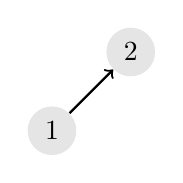
\begin{tikzpicture}[align=center]
	\tikzstyle{vertex} = [circle,fill=black!10]
	\tikzstyle{edge} = [->,thick]
	\node<1->[vertex] (n1) at (0,0) {1};
	\node<2->[vertex] (n2) at (1,1) {2};
	\draw<2->[edge] (n1)--(n2);
	\end{tikzpicture}
\end{frame}
\end{document}
